% !TEX root = ../main.tex

\section{Method}
\label{sec:method}

\begin{figure*}[t]
\centering
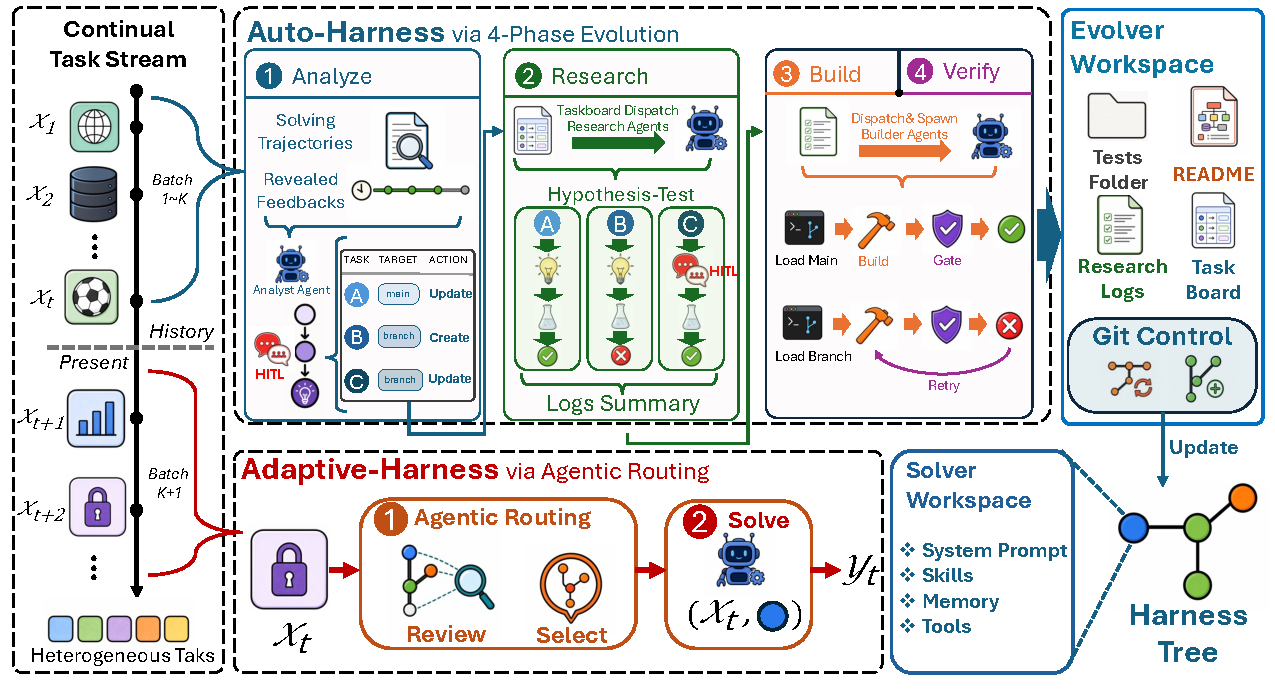
\includegraphics[width=0.95\textwidth]{figures/framework.pdf}
\caption{Overview of the Adaptive Auto-Harness system. \textbf{Bottom:} the multi-agent evolver constructs and refines a harness tree across cycles via four roles (Analyst $\to$ parallel Researchers $\to$ Builder $\to$ Verifier) with a persistent cross-cycle workspace and temporal-reveal feedback. \textbf{Top:} at solve time, a router agent reads each branch's workspace via \texttt{git show} and routes the incoming task $x_t$ to the most suitable branch. Two human-in-the-loop hooks (task-board steering and research-phase assistance) trigger only when the evolver's history lacks relevant signal.}
\label{fig:unified_pipeline}
\end{figure*}


\subsection{Problem Formulation}
\label{sec:method-setup}

We consider tasks arriving in an open-ended stream $x_1, x_2, \ldots, x_T$ with $x_t \sim P_t$, where $P_t$ is the task distribution at time $t$ and each $x_t$ has a fixed ground truth $y(x_t)$. The agent observes the history of prior experience $\Hist = \{(x_i, r_i, \tau_i)\}_{i=1}^{t-1}$, where $r_i$ is optionally the realized reward on task $x_i$ and $\tau_i$ is the agent's solving trajectory (actions, intermediate observations, tool calls). A \emph{harness} $C = \varphi(\Hist)$, with $|C| \leq K$, is a bounded representation (prompts, skills, memory, and tools) with capacity budget $K$, where $\varphi$ is the \emph{evolver}: the agentic system that automatically transforms historic experience into the harness. A solver agent then acts via the policy $a_t \sim \pi(a \mid x_t, C_t)$, where $\pi$ is the LLM-induced sampling distribution over actions conditioned on the task and harness.

\subsection{Analytical Framing}
\label{sec:framework}

The three deployment dimensions of \S\ref{sec:intro} surface concrete failures, but they do not by themselves identify what an evolver should fix. To pinpoint the root causes, we frame the problem analytically: we cast harness construction as a regret-minimization problem against an oracle reference, and decompose the regret into two complementary loss terms that map directly to actionable design axes.

\noindent\textbf{Utility and regret.}
We define the utility of a harness $C$ on a task $x_t$ as
\begin{equation}
\label{eq:utility}
V(C, x_t) = \mathbb{E}_{a \sim \pi(\cdot \mid x_t, C)}[r(a, y(x_t))],
\end{equation}
which is the expected reward of the harness-conditioned solver. The full-history utility is the corresponding ceiling under the capacity budget,
$V(\Hist, x_t) \,:=\, \sup_{\substack{C \,:\, |C| \leq K}} V(C, x_t)$,
that is, the best utility attainable by any bounded harness on $x_t$. The regret of the evolver-constructed harness is then
\begin{equation}
\label{eq:regret}
\text{Regret}(\varphi, x_t) = V(\Hist, x_t) - V(\varphi(\Hist), x_t) \geq 0,
\end{equation}
non-negative since $\varphi(\Hist)$ is one element of the supremum's domain. Operationally, this ceiling matches what a solver granted $\Hist$ directly, under the same compute and tool budget as $\varphi$, could attain by reconstructing any candidate harness on the fly.

\noindent\textbf{Solve-time optimal harness.}
Fix the evolver class $\Phi$ and define the solve-time optimal harness for a particular task:
\begin{equation}
\label{eq:cstar}
C^*_\Phi(x_t) = \arg\max_{\substack{C = \varphi(\Hist, x_t),\ \varphi \in \Phi \\ |C| \leq K}} V(C, x_t).
\end{equation}
This is an oracle reference: it is the best harness the evolver class $\Phi$ could produce if it were allowed to condition on the incoming task $x_t$ at solve time. A deployed evolver $\varphi$ commits to one harness $\varphi(\Hist)$ before $x_t$ is observed; using $C^*_\Phi$ as pivot between $V(\Hist, x_t)$ and $V(\varphi(\Hist), x_t)$ yields the following decomposition.

\begin{proposition}[Regret Decomposition]
\label{prop:decomp}
For any deployed evolver $\varphi \in \Phi$,
\begin{equation}
\label{eq:decomp}
\mathbb{E}_{x_t}[\text{Regret}(\varphi, x_t)] = \Levo(\Phi) + \Ladapt(\varphi),
\end{equation}
where
\begin{align}
\label{eq:losses}
\Levo(\Phi) &= \mathbb{E}_{x_t}\!\bigl[V(\Hist, x_t) - V(C^*_\Phi(x_t), x_t)\bigr],
\end{align}
\begin{align}
\Ladapt(\varphi)  &= \mathbb{E}_{x_t}\!\bigl[V(C^*_\Phi(x_t), x_t) - V(\varphi(\Hist), x_t)\bigr].
\end{align}
\end{proposition}

$\Levo$ is the \emph{evolution loss}: it reflects the evolver class $\Phi$'s capability gap, regardless of how many cycles the evolver runs. A single-agent prompt editor cannot produce multi-file infrastructure; that ceiling is structural, not a matter of effort. Reducing $\Levo$ therefore requires pursuing more capable evolver systems with access to broader control and feedbacks. $\Ladapt$ is the \emph{adaptation loss}: the oracle builds the optimal harness per task, but a deployed $\varphi$ commits to one harness before seeing $x_t$. Therefore, even with an optimal evolver system, $\Ladapt$ exists as long as task heterogeneity persists.

% Since $C^*_\Phi(x_t)$ dominates any fixed harness pointwise,
% \begin{equation}
% \label{eq:conditioning_gap}
% \mathbb{E}_{x_t}\!\bigl[V(C^*_\Phi(x_t), x_t)\bigr] \;\geq\; \max_{\varphi \in \Phi}\, \mathbb{E}_{x_t}\!\bigl[V(\varphi(\Hist), x_t)\bigr],
% \end{equation}
% with strict inequality whenever different tasks prefer different harnesses. 

\noindent\textbf{Human-in-the-loop as a third axis.}
The decomposition assumes $\Hist$ contains relevant signal for $x_t$. When it does not, the regret decomposition no longer applies; we address this case via a third axis outside $\Levo + \Ladapt$, the human-in-the-loop channel (\S\ref{sec:method-hitl}).


\subsection{Sustained Auto-Harness via Multi-Agent Evolution}
\label{sec:method-multi}

Reducing $\Levo$ requires expanding the evolution capability $\Phi$. We identify three structural limitations of prior single-agent evolvers: (i) evolution involves multiple complex subtasks that compete for a single context window, capping the complexity of constructible harnesses; (ii) the evolver lacks a proper feedback channel for unbounded streams where labels arrive asynchronously; (iii) without cross-cycle memory, the evolver's construction capability remains static and cannot compound with the growing history induced by unbounded streams (D1). We address each limitation in our multi-agent evolver (Figure~\ref{fig:unified_pipeline}, bottom panel):

\noindent\textbf{(1) Multi-agent with distinct roles and objectives.}
Because unbounded streams (D1) keep expanding the trajectory history an evolver must interpret, existing single-agent evolvers must fit analysis, research, implementation, and verification into one context window. We decompose evolution into four agents (Analyst $\to$ parallel Researchers $\to$ Builder $\to$ Verifier), each with a dedicated objective and full context budget. This eliminates the single-window bottleneck and lets parallel Researchers explore disjoint hypotheses without premature convergence.

\noindent\textbf{(2) Temporal-reveal feedback.}
Under unbounded streams (D1), labels arrive asynchronously (e.g., a prediction market resolves days after the trade). We implement a \emph{temporal-reveal gate} that surfaces each task's ground-truth label to the evolver only after its resolution date, providing a proper streaming feedback signal without leaking future information.

\noindent\textbf{(3) Persistent cross-cycle state.}
We provide the evolver with a dedicated workspace that persists across cycles, containing a task board (prioritised failure analysis), research logs (tested hypotheses with pass/fail verdicts), architecture documentation, and verification tests. This cross-cycle memory enables the evolver to refine its construction ability over time and build upon prior evolution experience rather than restarting from scratch.




\subsection{Solve-Time Adaptation via Harness-Tree Routing}
\label{sec:method-nav}

Reducing $\Ladapt$ requires the deployed harness to approximate $C^*_\Phi(x_t)$ across heterogeneous tasks. A naive approach would perform full adaptation at solve time, but this is expensive and unreliable under latency constraints. Therefore, we propose shifting the heavy adaptation work into evolution time, which requires the evolver to construct a \emph{branching harness tree} of specialised harnesses, and leave only a lightweight routing decision at solve time: selecting the most suitable harness branch given the current task context (Figure~\ref{fig:unified_pipeline}, top panel).

We instantiate this with two designs (Figure~\ref{fig:unified_pipeline}, top panel). \textbf{(1) Branching harness tree (built at evolution time).} The solver's workspace is a git repository. The evolver constructs regime-specific branches (e.g., \texttt{branch/crypto-classical}, \texttt{branch/binary-reversing}) during evolution, each carrying its own prompt, skills, and tool registry; git provides versioning, isolation, and lineage tracking across branches. \textbf{(2) Agentic routing (executed at solve time).} A router agent reads each branch's workspace via \texttt{git show} and selects the most suitable branch given $x_t$'s context; the solver then checks out that branch and executes.

\subsection{Human-in-the-Loop Channel}
\label{sec:method-hitl}

A failure mode orthogonal to the three deployment dimensions is \emph{experience insufficiency}: some tasks require inputs the evolver cannot synthesize from $\Hist$ alone, such as API credentials, novel-language sources, or proprietary endpoints not encountered before. In this regime, neither a richer evolver class $\Phi$ nor solve-time routing can recover what is absent from history; the regret decomposition cannot be reduced further because the full-history utility itself is low. We therefore introduce a third axis outside $\Levo + \Ladapt$: a human-in-the-loop channel that augments $\Hist$ with external input. Two structurally triggered hooks in the multi-agent pipeline (Figure~\ref{fig:unified_pipeline}) each provide a different form of human steering:
\noindent\textbf{(1) Task-board steering.}
After the Analyst updates the task board, a human may review it to add entries, adjust priorities, or supply domain guidance and source access. This proactively steers the subsequent research cycle with direction the evolver cannot derive from trajectories alone.
\noindent\textbf{(2) Interactive assistance during research.}
When a Researcher hits a barrier mid-execution that requires human intervention (e.g., an authentication wall), the hook prompts the human in real time. This reactively unblocks the research agent at the point of failure.
